\chapter{System Analysis}

The project hosts two kinds of roles: admins and users. 

The user will start a trip, save location and media, manipulate media share options and share all of contents on social media. Also user can download a shared content which that user has access privileges. User can follow the trip that downloaded. User can search other users; trips by location, name and trip type (walk, run, ride or car). User can organize team trips with other users. During the team trip users can see each other's location on the map.

The admins can view the content of trips or profile of users. They can also evaluate the complaints which has been created by users. They can decide whether they are right or not, if admins think the complaint that is created by users is right they can hide the content of profile,comment or the whole trip. They are also able to view the support messages.

The work model of the system is shown in Figure~\ref{fig:system_diagram} and user roles shown in Figure \ref{fig:roles}.

\begin{figure}[!htbp]
\centering
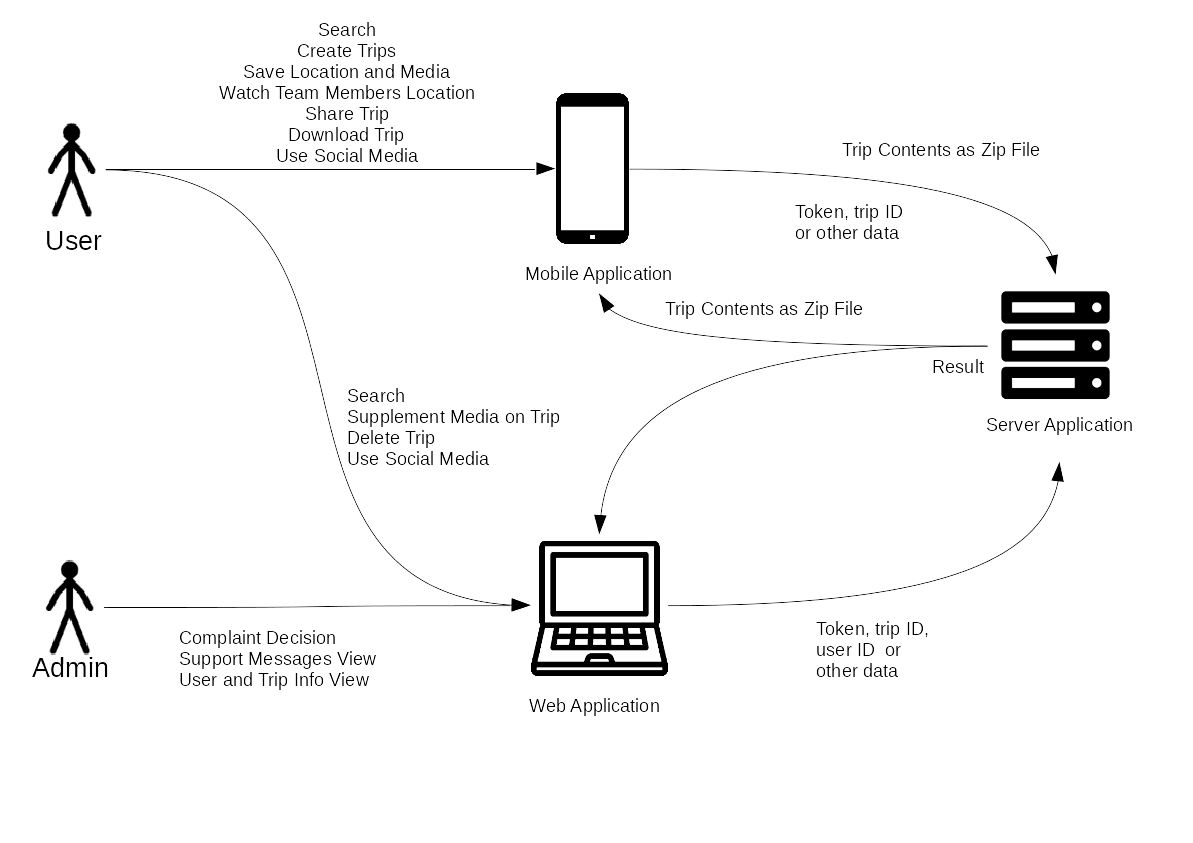
\includegraphics[width=\textwidth]{projectChapters/images/system_diagram.png}
\caption{System Schema}
\label{fig:system_diagram}
\end{figure}

\begin{figure}[!htbp]
\centering
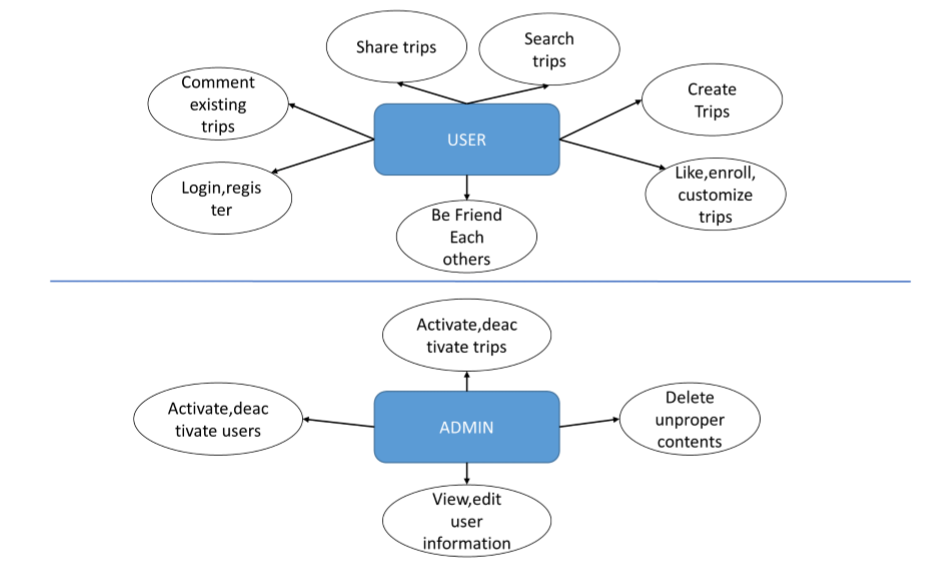
\includegraphics[width=\textwidth]{projectChapters/images/ER.png}
\caption{User Roles}
\label{fig:roles}
\end{figure}
\newpage
In designed system while user creating personal trips, user can pause or continue location track. User can add media files when location track enabled. User can share trip after trip finished. Workflow schema for creating a personal trip shown in Figure \ref{fig:personalTripWorkflow}. 

\begin{figure}[!htbp]
\centering
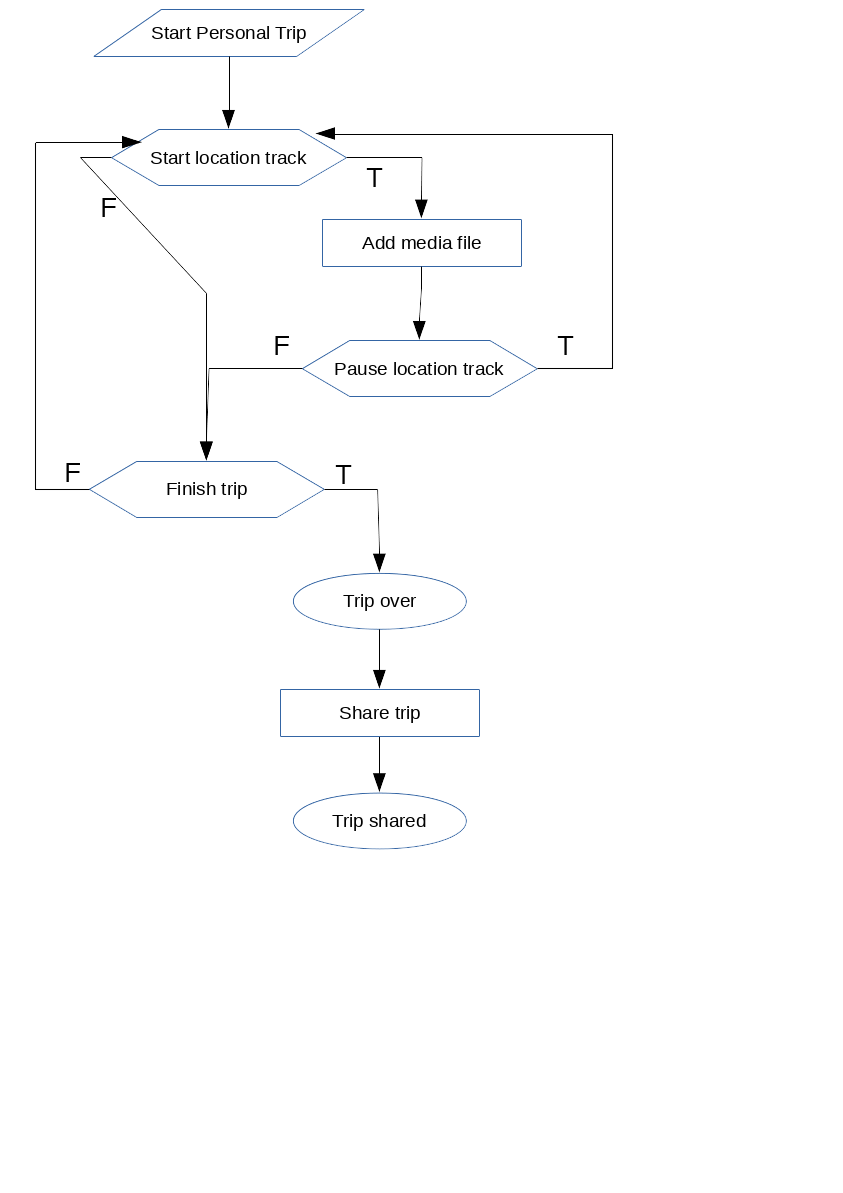
\includegraphics[width=\textwidth]{projectChapters/images/personalTripWorkflow.png}
\caption{Workflow Schema For Creating Personal Trip}
\label{fig:personalTripWorkflow}
\end{figure}

While creating team trips user must choose team members from his/her friend list before starting trip. When user starts trip user is selected as team leader and all of choosen member(s) will get a trip invitation notification for the trip. If member accepts invitation he/she will be in this team trip. During team trip all of the features of personal trip will be available. In addition, location sharing function with other team member(s) will be available and locations of team members will be shown on the map asynchronously. When trip finishes team leader may share the trip and selected media contents. After words other team members can only add their personal media to the published trip. Workflow schema for creating a team trip shown in Figure \ref{fig:teamTripWorkflow}.

\begin{figure}[!htbp]
\centering
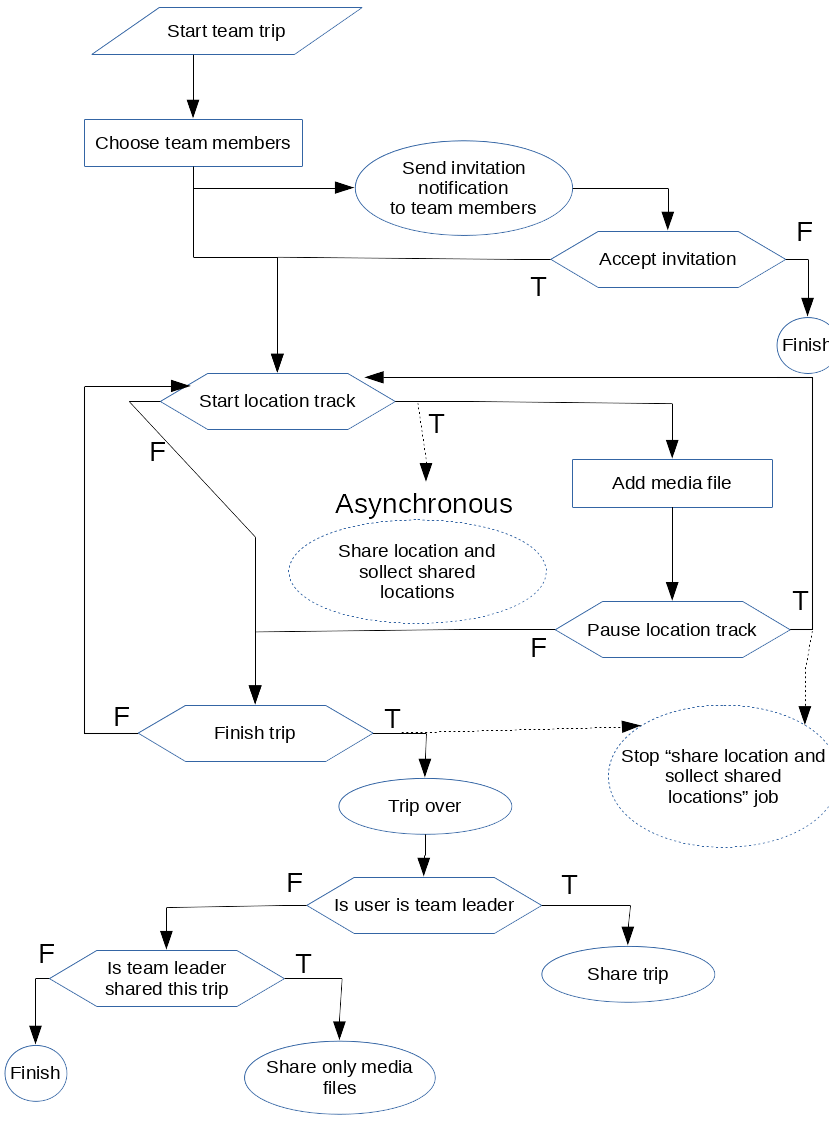
\includegraphics[ height = 40em ]{projectChapters/images/teamTripWorkflow.png}
\caption{Workflow Schema For Creating Team Trip}
\label{fig:teamTripWorkflow}
\end{figure}